\documentclass[UTF8,a4paper]{article}
\usepackage{ctex}
\usepackage{amsmath}
\usepackage{amssymb}
\usepackage{graphicx}
\usepackage{fancyhdr}
\usepackage{CJK}
\usepackage{chngpage}
\usepackage{url}
\setCJKmainfont{宋体}
\usepackage{listings}
\usepackage{xcolor}
\usepackage[numbers,sort&compress]{natbib}
\usepackage{xpatch}
\usepackage{geometry}
\xpatchcmd{\thebibliography}{\section*}{\section}{}{}
\geometry{left=2.9cm,right=2.9cm,top=3cm,bottom=2.9cm}

\definecolor{CPPLight}  {HTML} {686868}
\definecolor{CPPSteel}  {HTML} {888888}
\definecolor{CPPDark}   {HTML} {262626}
\definecolor{CPPBlue}   {HTML} {4172A3}
\definecolor{CPPGreen}  {HTML} {487818}
\definecolor{CPPBrown}  {HTML} {A07040}
\definecolor{CPPRed}    {HTML} {AD4D3A}
\definecolor{CPPViolet} {HTML} {7040A0}
\definecolor{CPPGray}  {HTML} {B8B8B8}


\lstset{
	columns=fixed,       
	numbers=left,                                        % 在左侧显示行号
	frame=none,                                          % 不显示背景边框
	backgroundcolor=\color[RGB]{245,245,244},            % 设定背景颜色
	keywordstyle=\color[RGB]{40,40,255},                 % 设定关键字颜色
	numberstyle=\footnotesize\color{darkgray},           % 设定行号格式
	commentstyle=\it\color[RGB]{0,96,96},                % 设置代码注释的格式
	basicstyle=\small,
	stringstyle=\rmfamily\slshape\color[RGB]{128,0,0},   % 设置字符串格式
	showstringspaces=false,                              % 不显示字符串中的空格
	language=c++,                                        % 设置语言
	morekeywords={alignas,continute,friend,register,true,alignof,decltype,goto,
		reinterpret_cast,try,asm,defult,if,return,typedef,auto,delete,inline,short,
		typeid,bool,do,int,signed,typename,break,double,long,sizeof,union,case,
		dynamic_cast,mutable,static,unsigned,catch,else,namespace,static_assert,using,
		char,enum,new,static_cast,virtual,char16_t,char32_t,explict,noexcept,struct,
		void,export,nullptr,switch,volatile,class,extern,operator,template,wchar_t,
		const,false,private,this,while,constexpr,float,protected,thread_local,
		const_cast,for,public,throw,std},
	emph={map,set,multimap,multiset,unordered_map,unordered_set,
		unordered_multiset,unordered_multimap,vector,string,list,deque,
		array,stack,forwared_list,iostream,memory,shared_ptr,unique_ptr,
		random,bitset,ostream,istream,cout,cin,endl,move,default_random_engine,
		uniform_int_distribution,iterator,algorithm,functional,bing,numeric,},
	emphstyle=\color{CPPViolet}, 
}



%opening
\title{实验二 分组密码算法DES}
\author{1611531-信息安全-刘新慧}
\date{}
\begin{document}

\maketitle

\begin{abstract}
通过用DES算法对实际的数据进行加密和解密来深刻了解DES的运行原理。\par 
\end{abstract}
\tableofcontents
\newpage

	\section{实验原理}
分组密码是一种对称密码体制,其特点是在明文加密和密文解密的过程中,信息都是按照固定长度分组后进行处理的。在分组密码的发展历史中,曾出现了许多优秀的算法,包括DES,IDEA,AES,Safer++等等。下面以DES算法为例介绍分组密码算法的实现机制。\par
DES算法将明文分成64位大小的众多数据块,即分组长度为64位。同时用56位密钥对64位明文信息加密,最终形成64位的密文。如果明文长度不足64位,即将其扩展为64位(如补零等方法)。具体加密过程首先是将输入的数据进行初始置换(IP),即将明文M中数据的排列顺序按一定的规则重新排列,生成新的数据序列,以打乱原来的次序。然后将变换后的数据平分成左右两部分,左边记为L0,右边记为R0,然后对R0实行在子密钥(由加密密钥产生)控制下的变换f,结果记为f(R0,K1),再与L0做逐位异或运算,其结果记为R1,R0则作为下一轮的L1。如此循环16轮,最后得到L16、R16,再对L16、R16实行逆初始置换IP-1,即可得到加密数据。解密过程与此类似,不同之处仅在于子密钥的使用顺序正好相反。DES全部16轮的加密过程如图1所示:\par 
		\begin{figure}[!ht]
	
	\centering
	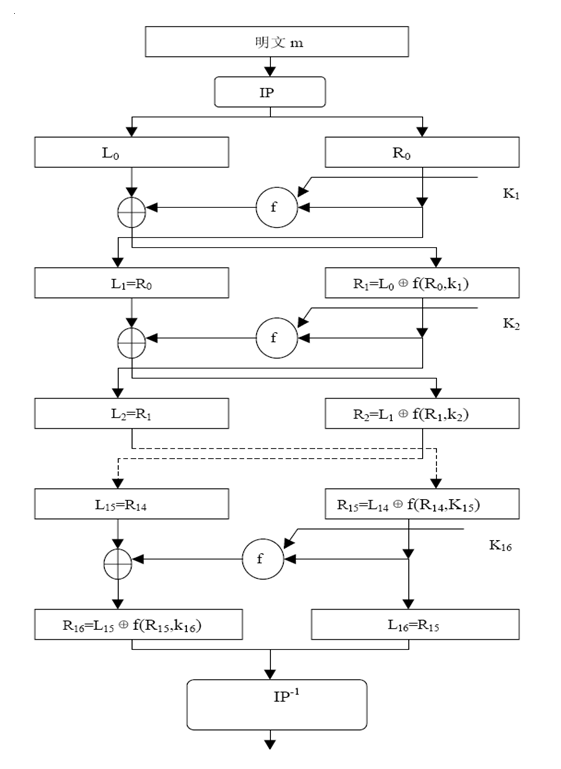
\includegraphics[width=0.67\textwidth]{1-1.PNG}
	\caption{DES加密/解密流程}
	\label{fig:1-1}
\end{figure}


DES的加密算法包括3个基本函数:\par 
1.	初始置换IP\par 
它的作用是把输入的64位数据块的排列顺序打乱,每位数据按照下面的置
换规则重新排列,即将第58位换到第一位,第50位换打第2位,…,依次类推。置换后的64位输出分为L0 、R0(左、右)两部分,每部分分别为32位。\par 
\begin{center}
	 58 50 42 34 26 18 10 2 60 52 44 36 28 20 12 4\\
	62 54 46 38 30 22 14 6 64 56 48 40 32 24 16 8\\
	57 49 41 33 25 17 9  1 59 51 43 35 27 19 11 3\\
	61 53 45 37 29 21 13 5 63 55 47 39 31 23 15 7\par
	\end{center}
    R0和K1经过f(R0,K1)变换后的输出结果,再和L0进行异或运算,输出结果位R1,R0则赋给L1。L1和R1同样再做类似运算生成L2和R2,…,经过16次运算后生成L16和R16。\par 	
 2.f 函数\par 
f 函数是多个置换函数和替代函数的组合函数,它将32位比特的输入变换为32位的输出,如图2所示。Ri经过扩展运算E变换后扩展为48位的E(Ri),与 进行异或运算后输出的结果分成8组,每组6比特。每一组再经过一个S盒(共8个S盒)运算转换为4位,8个4位合并为32位后再经过P变换输出为32位的 。其中,扩展运算E与置换P主要作用是增加算法的扩散效果。\par 
		\begin{figure}[!ht]
	
	\centering
	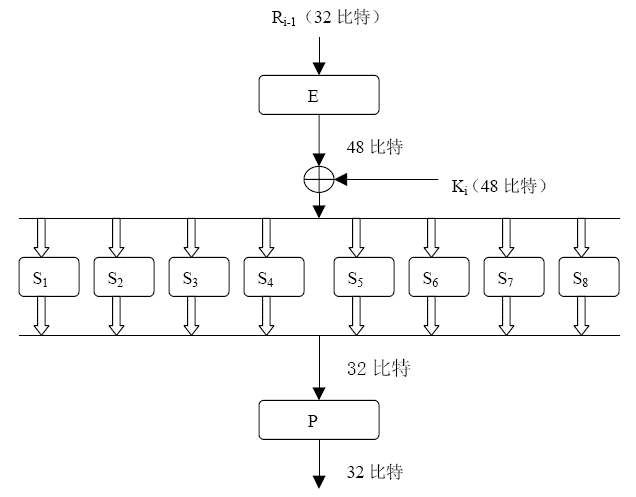
\includegraphics[width=0.75\textwidth]{1-2.PNG}
	\caption{f函数原理图}
	\label{fig:1-2}
\end{figure}
3.逆初始置换IP-1
\par 它将L16和R16作为输入,进行逆初始置换得到密文输出。逆初始置换是初始
置换的逆运算,置换规则如下所列:\par 

\begin{center}
40,8,48,16,56,24,64,32,39,7,47,15,55,23,63,31\\
38,6,46,14,54,22,62,30,37,5,45,13,53,21,61,29\\
36,4,44,12,52,20,60,28,35,3,43,11,51,19,59,27\\
34,2,42,10,50,18,58,26,33,1,41,9, 49,17,57,25\par 

\end{center}
DES的加密算法中除了上面介绍的3个基本函数,还有一个非常重要的功能模块,即子密钥的生成模块,具体子密钥的产生流程图如图3所示。输入的初始密钥值为64位,但DES算法规定,其中第8、16、…、64位为奇偶校验位,不参予DES的运算。所以,实际可用位数只有56位,经过缩小选择位表1(表1-2)即密钥置换PC-1的变换后,初始密钥的位数由64位变成了56位,将其平分位两部分C0,D0。然后分别进行第一次循环左移,得到C1和D1,将C1(28位)、D1(28位)合并后得到56位的输出结果,再经过压缩置换PC-2(表1-3),从而得到了密钥K1(48位)。依次类推,便可得到K2、…、K16。需要注意的是,16次循环左移对应的左移位数要依据表1-1的规则进行。
		\begin{figure}[!ht]
	
	\centering
	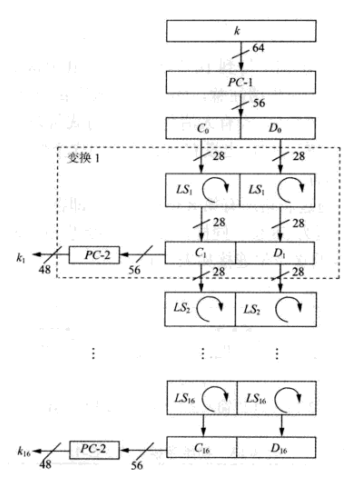
\includegraphics[width=0.6\textwidth]{1-3.PNG}
	\caption{子密钥的生成流程}
	\label{fig:1-3}
\end{figure}

		\begin{figure}[!ht]
	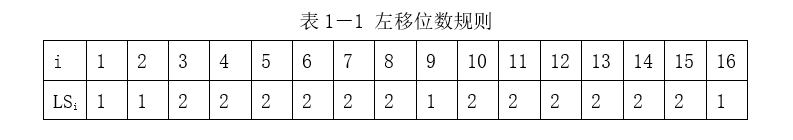
\includegraphics[width=1.0\textwidth]{c1.PNG}
\end{figure}

		\begin{figure}[!ht]
	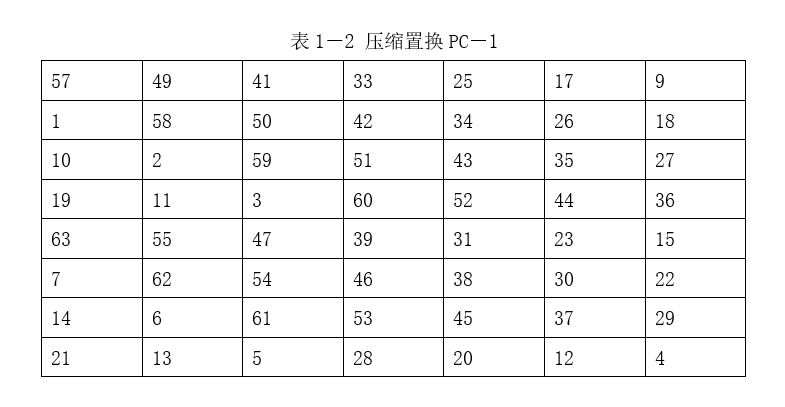
\includegraphics[width=1.0\textwidth]{c2.PNG}
\end{figure}


		\begin{figure}[!ht]
	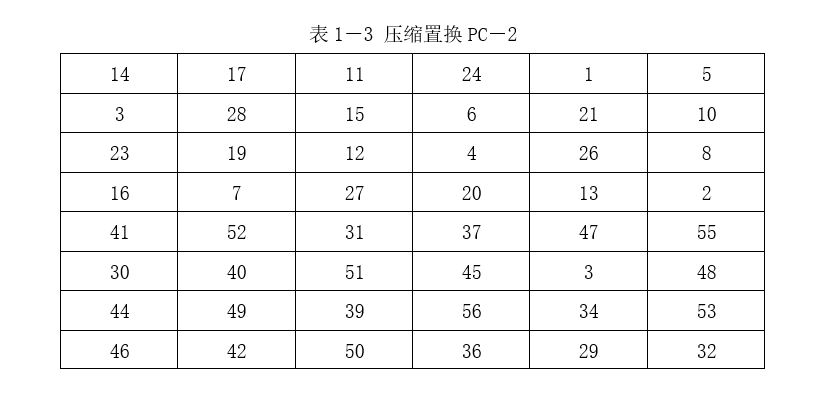
\includegraphics[width=1.0\textwidth]{c3.PNG}
\end{figure}


	\section{实验内容和步骤}
1.算法分析:
对课本中DES算法进行深入分析,对初始置换、E扩展置换,S盒代换、
轮函数、密钥生成等环节要有清晰的了解,并考虑其每一个环节的实现过程。\par 
2.	DES实现程序的总体设计:在第一步的基础上,对整个DES加密函数的
实现进行总体设计,考虑数据的存储格式,参数的传递格式,程序实现的总体层次等,画出程序实现的流程图。   \par 
3.	在总体设计完成后,开始具体的编码,在编码过程中,注意要尽量使用
高效的编码方式。\par 
4.	利用3中实现的程序,对DES的密文进行雪崩效应检验。即固定密钥,
仅改变明文中的一位,统计密文改变的位数;固定明文,仅改变密钥中的一位,统计密文改变的位数。\par \section{流程图}
整体流程图如下:\par 
	\begin{center}
	
	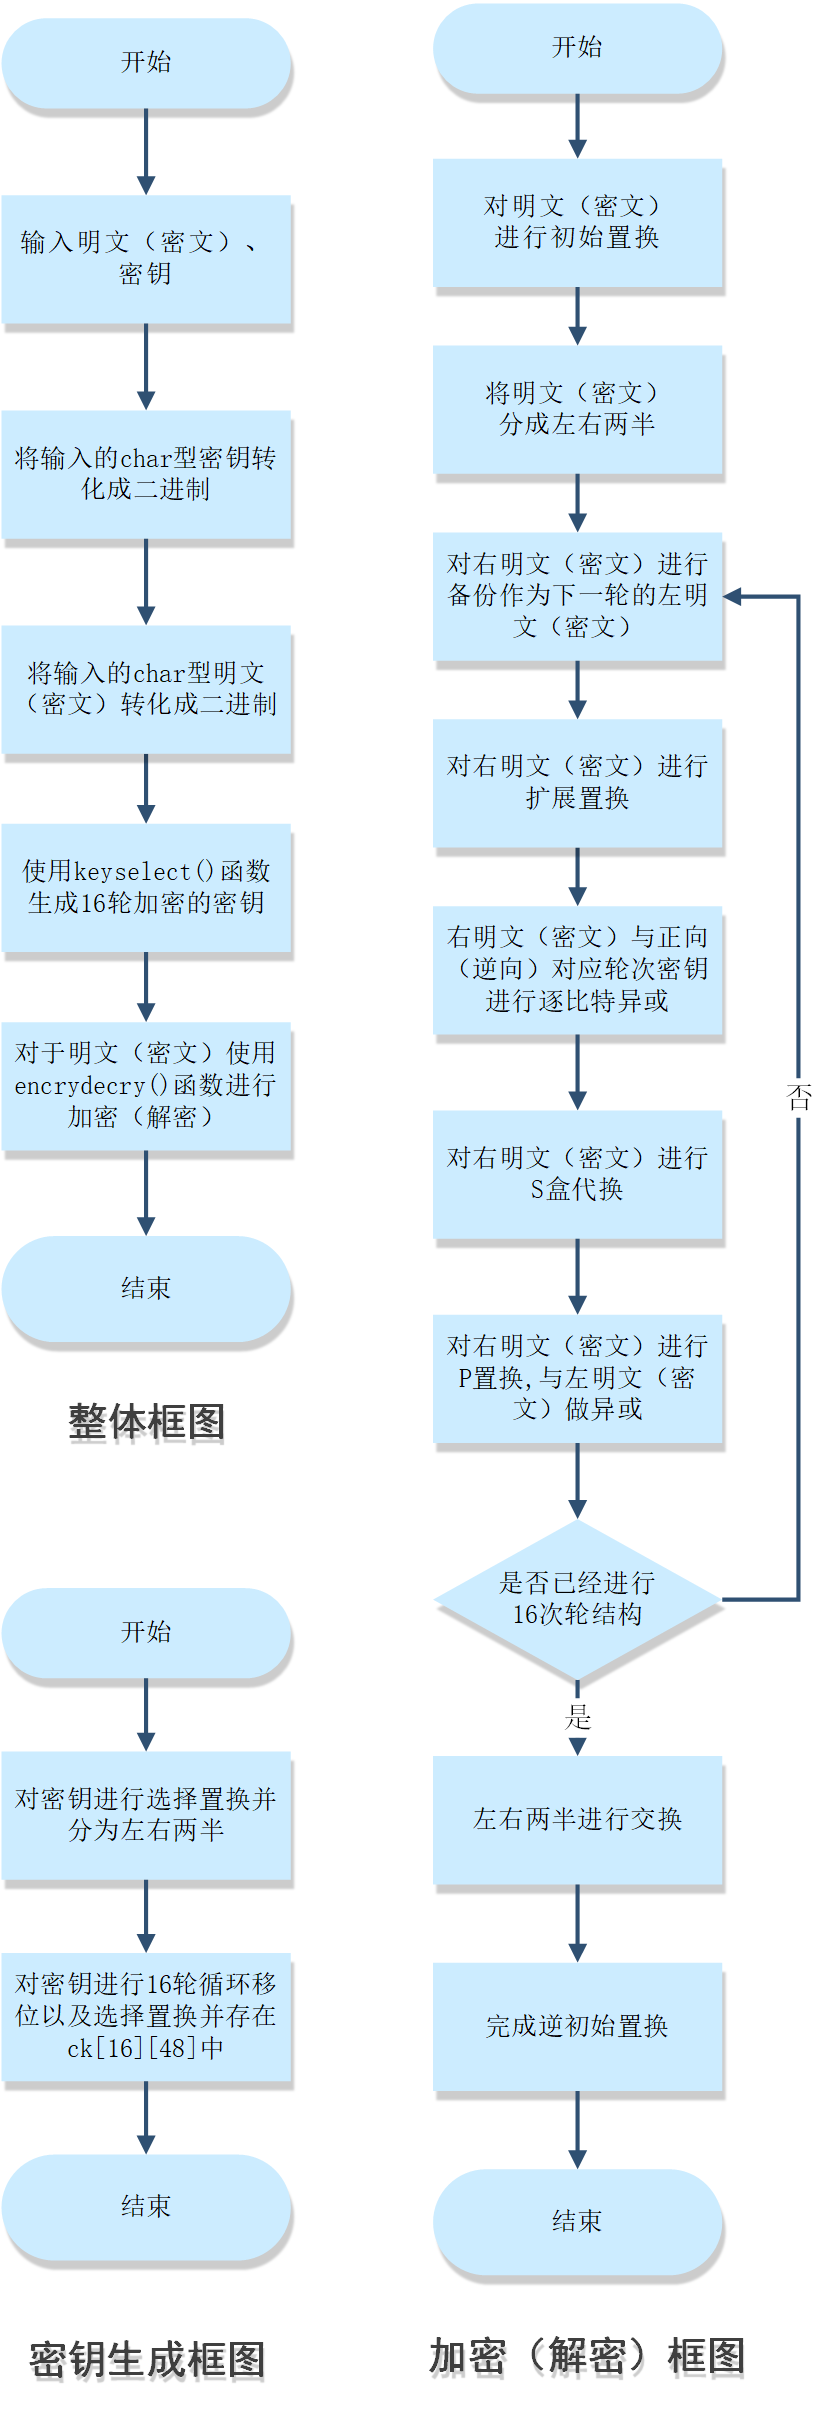
\includegraphics[width=0.48\textwidth]{image.PNG}

\end{center}

	\section{实验结果}
代码运行后显示如下:\par 
		\begin{figure}[!ht]
	
	\centering
	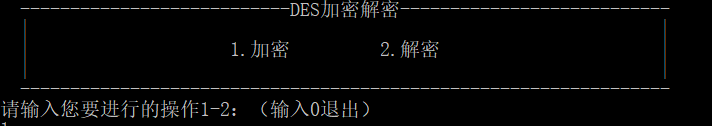
\includegraphics[width=1.0\textwidth]{p1.PNG}
	\caption{初始界面}
	\label{fig:p1}
\end{figure}
进行加密:\par 
		\begin{figure}[!ht]
	
	\centering
	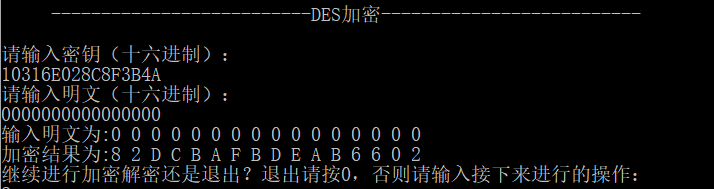
\includegraphics[width=1.0\textwidth]{p2.PNG}
	\caption{加密结果}
	\label{fig:p2}
\end{figure}
进行解密:\par 
		\begin{figure}[!ht]
	
	\centering
	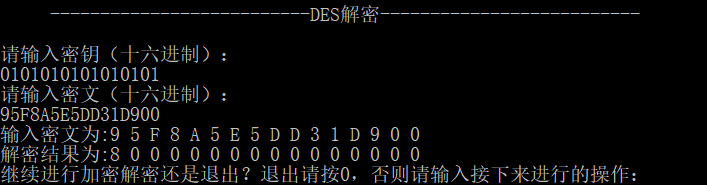
\includegraphics[width=1.0\textwidth]{p3.PNG}
	\caption{解密结果}
	\label{fig:p3}
\end{figure}
	\section{雪崩效应检验}
写代码进行检验:\par
改变密文,计算密文修改的平均位数,实验结果如下图:\par 
		\begin{figure}[!ht]
	
	\centering
	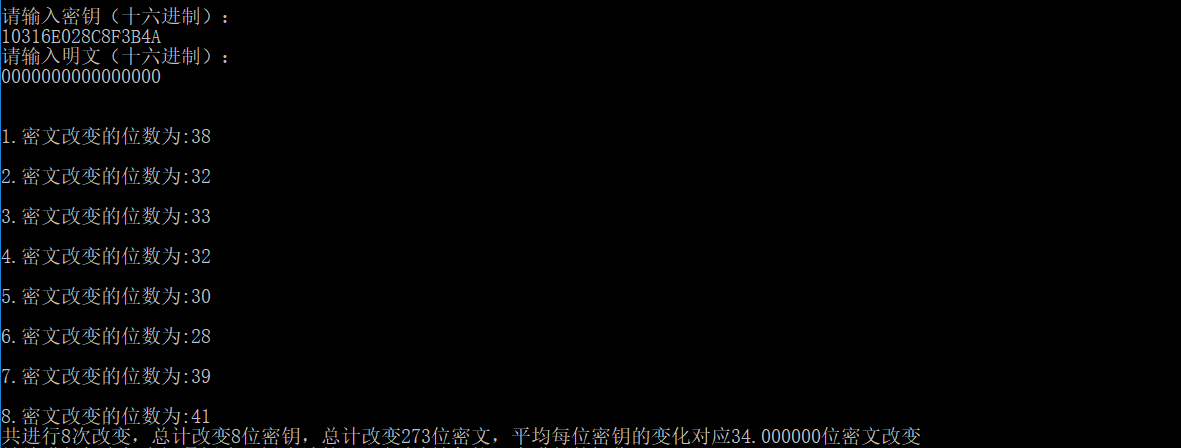
\includegraphics[width=1.0\textwidth]{miyao.PNG}
	\label{fig:miyao}
\end{figure}
\newpage
改变明文,计算密文修改的平均位数,实验结果如下图:\par 
		\begin{figure}[!ht]
	
	\centering
	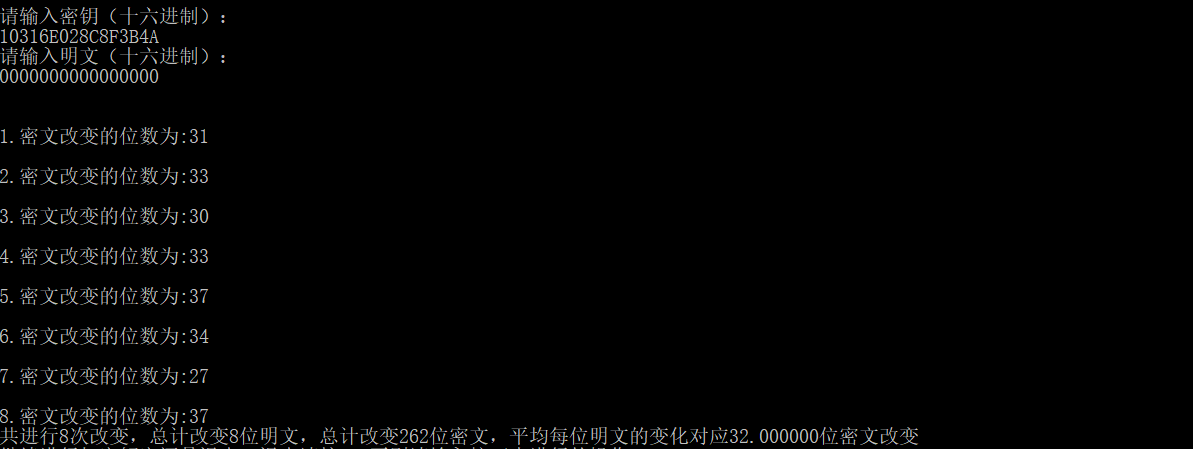
\includegraphics[width=1.0\textwidth]{mingwen.PNG}
	\label{fig:mingwen}
\end{figure}




\end{document}
